\documentclass[border=1pt]{standalone}
\usepackage{tikz}
\usepackage{luatexja}
\usetikzlibrary{backgrounds}

\begin{document}
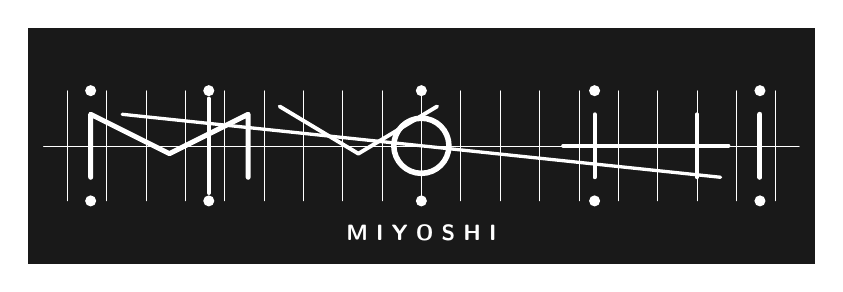
\begin{tikzpicture}[line width=1.4pt, line cap=round, line join=round]
    % 黒背景の設定
    \begin{scope}[on background layer]
        \fill[black!90] (-5.0, -1.5) rectangle (5.0, 1.5);
    \end{scope}

    % 全体の色を白(white)に変更
    \begin{scope}[white]
        % 精密グリッド (薄い白)
        \begin{scope}[white!20, line width=0.2pt]
            \foreach \x in {-4.5, -4.0, ..., 4.5} \draw (\x, -0.7) -- (\x, 0.7);
            \draw (-4.8, 0) -- (4.8, 0);
        \end{scope}

        % MIYOSHI 構造
        \draw[line width=1.8pt] (-4.2, -0.4) -- (-4.2, 0.4) -- (-3.2, -0.1) -- (-2.2, 0.4) -- (-2.2, -0.4); % M
        \draw (-2.7, -0.6) -- (-2.7, 0.6); % I
        \draw (-1.8, 0.5) -- (-0.8, -0.1) -- (0.2, 0.5); % Y
        \draw[line width=2pt] (0, 0) circle (0.35); % O
        \draw[line width=1.2pt] (-3.8, 0.4) -- (3.8, -0.4); % S (鋭い一閃)
        \draw (2.2, -0.4) -- (2.2, 0.4); % H
        \draw (3.5, -0.4) -- (3.5, 0.4);
        \draw (1.8, 0) -- (3.9, 0); % H横棒
        \draw[line width=1.8pt] (4.3, -0.4) -- (4.3, 0.4); % I

        % 装飾点と端
        \foreach \x in {-4.2, -2.7, 0, 2.2, 4.3} {
            \fill[white] (\x, 0.7) circle (2pt);
            \fill[white] (\x, -0.7) circle (2pt);
        }
        
        % サブテキスト
        \node[font=\sffamily\bfseries, scale=0.8] at (0, -1.1) {M I Y O S H I};
    \end{scope}
\end{tikzpicture}
\end{document}
